\subsection{Теорема о среднем. Следствия из теоремы о среднем}

В данном билете рассматриваются утверждения, позволяющие оценить значение определенного интеграла через значения функции внутри промежутка интегрирования. Эти теоремы имеют важное значение для оценки погрешностей и доказательства фундаментальных формул анализа.

\subsubsection*{1. Теорема о среднем для интегрируемых функций}

Лектор отмечает, что это утверждение является аналогом теоремы Лагранжа для интегралов. Оно связывает интеграл от функции с её точными гранями на отрезке.

\begin{theorem}
Пусть функция $f(x)$ интегрируема на отрезке $[a, b]$. Пусть $m$ — инфимум, а $M$ — супремум функции $f(x)$ на этом отрезке:
\[ m = \inf_{x \in [a, b]} f(x), \quad M = \sup_{x \in [a, b]} f(x) \]
Тогда существует такое число $\mu \in [m, M]$, что:
\[ \int\limits_a^b f(x) dx = \mu (b - a) \]
\end{theorem}

\begin{tcolorbox}[title=Доказательство, breakable]
Рассмотрим случай $a < b$ (случай $a = b$ тривиален, так как обе части равны нулю).

1. По свойству оценки интеграла через грани функции на отрезке $[a, b]$ выполняется неравенство:
\[ m(b - a) \le \int\limits_a^b f(x) dx \le M(b - a) \]

2. Разделим все части неравенства на положительную величину $(b - a)$:
\[ m \le \frac{1}{b - a} \int\limits_a^b f(x) dx \le M \]

3. Обозначим величину в центре через $\mu$:
\[ \mu = \frac{1}{b - a} \int\limits_a^b f(x) dx \]
По построению число $\mu$ заключено в пределах $[m, M]$. 

4. Из определения $\mu$ сразу следует искомое равенство:
\[ \int\limits_a^b f(x) dx = \mu (b - a) \]

В случае $a > b$ доказательство аналогично: при перемене пределов интегрирования интеграл умножается на $-1$, и разность $(b-a)$ также меняет знак, в результате чего равенство сохраняется.
\end{tcolorbox}

\subsubsection*{2. Следствие для непрерывных функций (Первая теорема о среднем)}

Если наложить на функцию условие непрерывности, то значение $\mu$ обязательно будет достигаться функцией в некоторой точке $\xi$.

\begin{consequence}
Если функция $f(x)$ непрерывна на отрезке $[a, b]$, то существует такая точка $\xi \in [a, b]$, что:
\[ \int\limits_a^b f(x) dx = f(\xi)(b - a) \]
\end{consequence}

\begin{tcolorbox}[title=Доказательство, breakable]
1. Так как $f(x)$ непрерывна на отрезке $[a, b]$, то она по теореме Вейерштрасса ограничена и достигает своих точных граней $m$ и $M$ (минимума и максимума).
2. По предыдущей теореме (для интегрируемых функций) существует число $\mu \in [m, M]$, такое что $\int_a^b f(x) dx = \mu (b - a)$.
3. Согласно теореме Больцано — Коши о промежуточном значении, непрерывная функция на отрезке принимает все значения между своим минимумом и максимумом. 
4. Следовательно, для любого $\mu \in [m, M]$ найдется такая точка $\xi \in [a, b]$, в которой $f(\xi) = \mu$. 
5. Подставляя $f(\xi)$ вместо $\mu$ в формулу из основной теоремы, получаем требуемое.
\end{tcolorbox}

\subsubsection*{3. Геометрический смысл}

Геометрический смысл теоремы о среднем (для положительной функции) заключается в том, что площадь криволинейной трапеции под графиком $f(x)$ на отрезке $[a, b]$ равна площади некоторого прямоугольника с тем же основанием $[a, b]$. Высота этого прямоугольника равна значению функции в некоторой промежуточной точке $\xi$.

%\begin{center}
%\includegraphics[width=0.6\textwidth]{mean_value_geometry.png}
% На рисунке изображен график функции f(x) на [a, b], 
% отмечена точка xi на оси Ox и значение f(xi). 
% Заштрихован прямоугольник высотой f(xi), площадь которого 
% совпадает с площадью под кривой.
%\end{center}

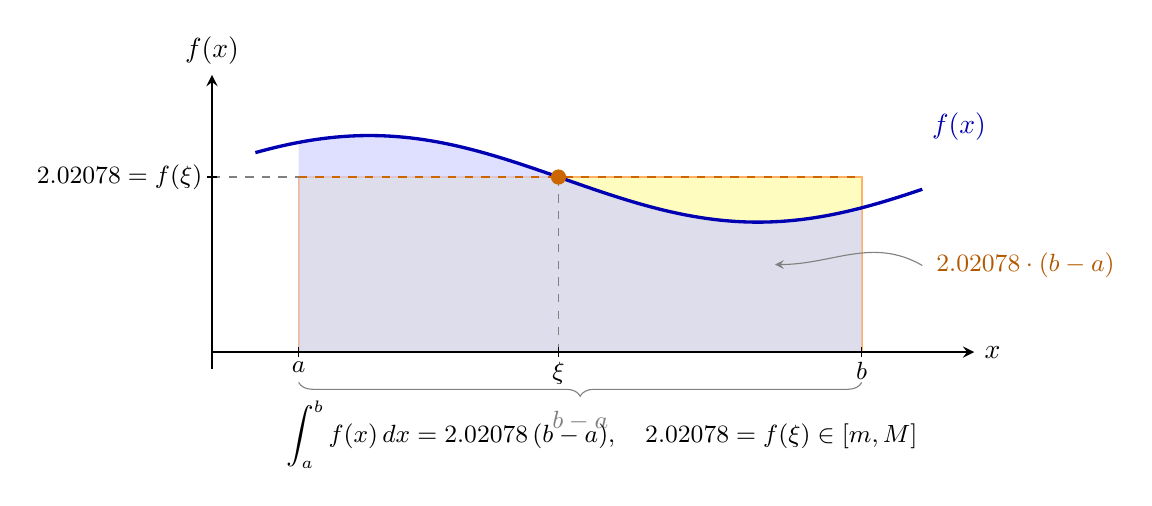
\begin{tikzpicture}[>=stealth, scale=1.1]
 
% ИСПРАВЛЕНО: #1 вместо \x
\pgfmathdeclarefunction{ff}{1}{%
  \pgfmathparse{0.5*sin(deg(#1*0.7+0.3))+2.0}%
}
 
\def\xa{1.0}
\def\xb{7.5}
\def\xxi{4.0}
\pgfmathsetmacro{\mu}{ff(\xxi)}
 
%--- Прямоугольник «среднее» ---
\fill[yellow!25,draw=orange!60,line width=0.8pt]
  (\xa,0) rectangle (\xb,\mu);
 
%--- Область под кривой ---
\fill[blue!18,opacity=0.7,domain=\xa:\xb,samples=80]
  plot(\x,{ff(\x)}) -- (\xb,0) -- (\xa,0) -- cycle;
 
%--- Кривая ---
\draw[blue!70!black,very thick,domain=0.5:8.2,samples=100]
  plot(\x,{ff(\x)});
 
%--- Горизонтальная линия на высоте μ ---
\draw[orange!80!black,dashed,thick] (\xa,\mu)--(\xb,\mu);
 
%--- Вертикаль из ξ ---
\pgfmathsetmacro{\fxi}{ff(\xxi)}
\draw[gray,dashed] (\xxi,0)--(\xxi,\fxi);
\fill[orange!80!black] (\xxi,\fxi) circle(2.5pt);
 
%--- Оси ---
\draw[->,thick] (0,0)--(8.8,0) node[right]{$x$};
\draw[->,thick] (0,-0.2)--(0,3.2) node[above]{$f(x)$};
 
%--- Метки ---
\foreach \xp/\lab in {\xa/{$a$},\xb/{$b$},\xxi/{$\xi$}}{
  \draw (\xp,0.06)--(\xp,-0.06);
  \node[below,font=\small] at (\xp,0) {\lab};
}
 
%--- f(ξ) = μ на оси Y ---
\draw[dashed,gray,thin] (0,\mu)--(\xa,\mu);
\draw (0.06,\mu)--(-0.06,\mu);
\node[left,font=\small] at (0,\mu){$\mu=f(\xi)$};
 
%--- Скобка (b-a) ---
\draw[decorate,decoration={brace,amplitude=5pt,mirror},gray]
  (\xa,-0.35)--(\xb,-0.35)
  node[midway,below=7pt,font=\small]{$b-a$};
 
%--- Стрелка к прямоугольнику ---
\draw[->,gray,thin] (8.2,1.0) to[out=150,in=0] (6.5,\mu/2);
\node[right,font=\small,orange!70!black] at (8.25,1.0){$\mu\cdot(b-a)$};
 
%--- Подпись ---
\node[font=\small] at (4.5,-0.95)
  {$\displaystyle\int_a^b f(x)\,dx=\mu\,(b-a),
    \quad \mu=f(\xi)\in[m,M]$};
 
\node[blue!70!black,font=\itshape,right] at (8.2,2.6){$f(x)$};
 
\end{tikzpicture}

\subsubsection*{4. Обобщенная теорема о среднем (без доказательства)}

Лектор упоминает более общую форму, когда под интегралом стоит произведение двух функций.

\begin{theorem}
Пусть функции $f(x)$ и $g(x)$ интегрируемы на $[a, b]$, причем функция $g(x)$ сохраняет знак на этом отрезке (либо везде $g(x) \ge 0$, либо везде $g(x) \le 0$). Тогда существует число $\mu \in [m, M]$, такое что:
\[ \int\limits_a^b f(x)g(x) dx = \mu \int\limits_a^b g(x) dx \]
Если при этом $f(x)$ непрерывна, то $\mu = f(\xi)$ для некоторого $\xi \in [a, b]$.
\end{theorem}
